\placelogofalse
\begin{frame}{Astrophysics + Moving Voronoi Mesh}
  \begin{columns}
  \column{0.48\linewidth}
  \begin{outline}
    \1 Arepo  \cite{Springel2010Pur} (2010), solve MHD
    \2 Moving mesh 
    \2 Generator points move with Fluid
    \2 Re-mesh with Delaunay 
    \2 Create Dual / Voronoi Cells 
    \2 Control Volumes for Finite Volume scheme
    \1 How to increase accuracy? \cite{Gaburro2020High}(2020)
  \end{outline}

  \column{0.48\linewidth}

  \begin{center}
    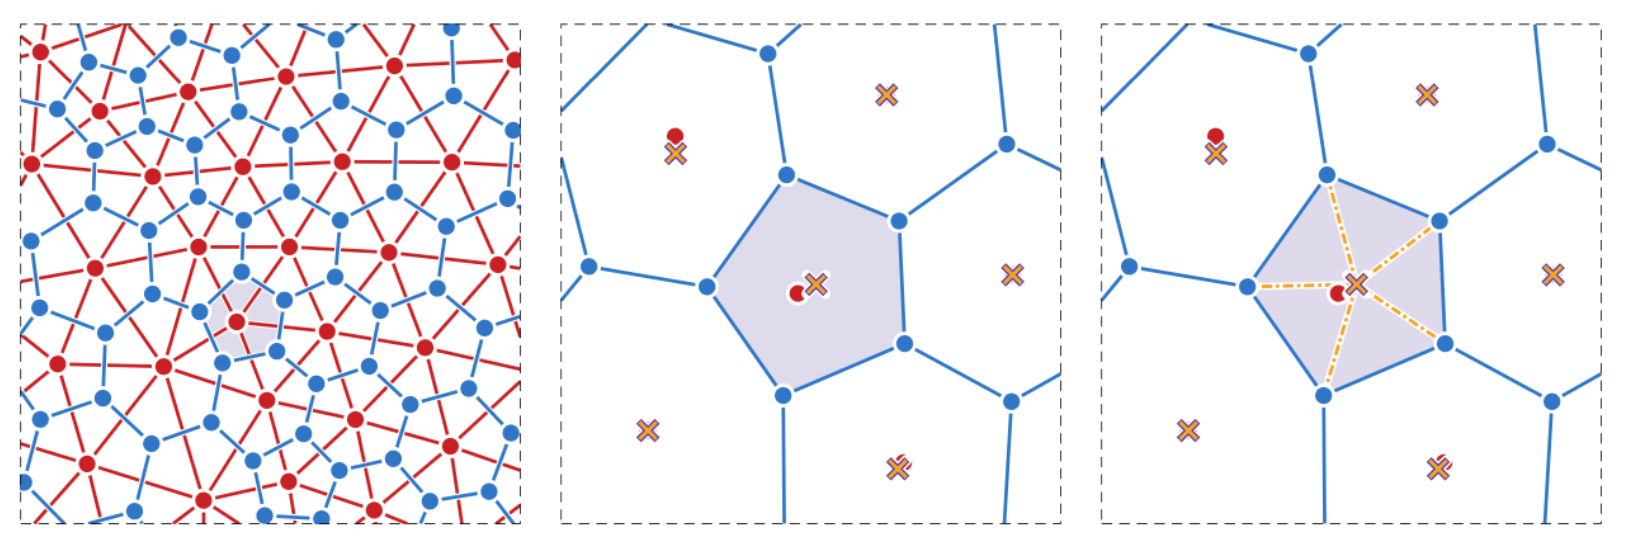
\includegraphics[width=0.9\linewidth]{voronoi.png}

    \vspace{0.2cm}


    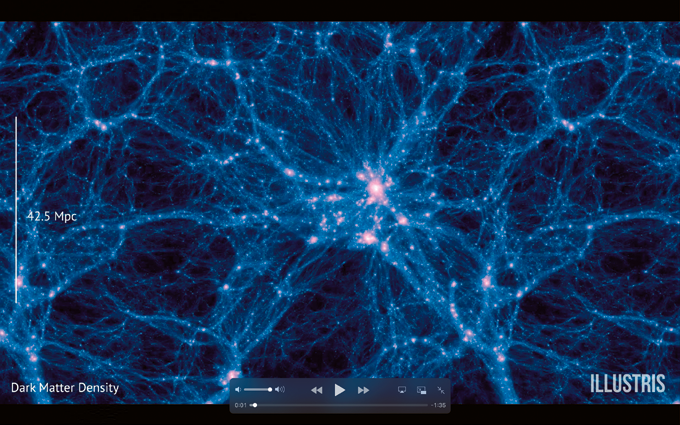
\includegraphics[width=0.6\linewidth]{illustris.png}

    \vspace{0.2cm}

    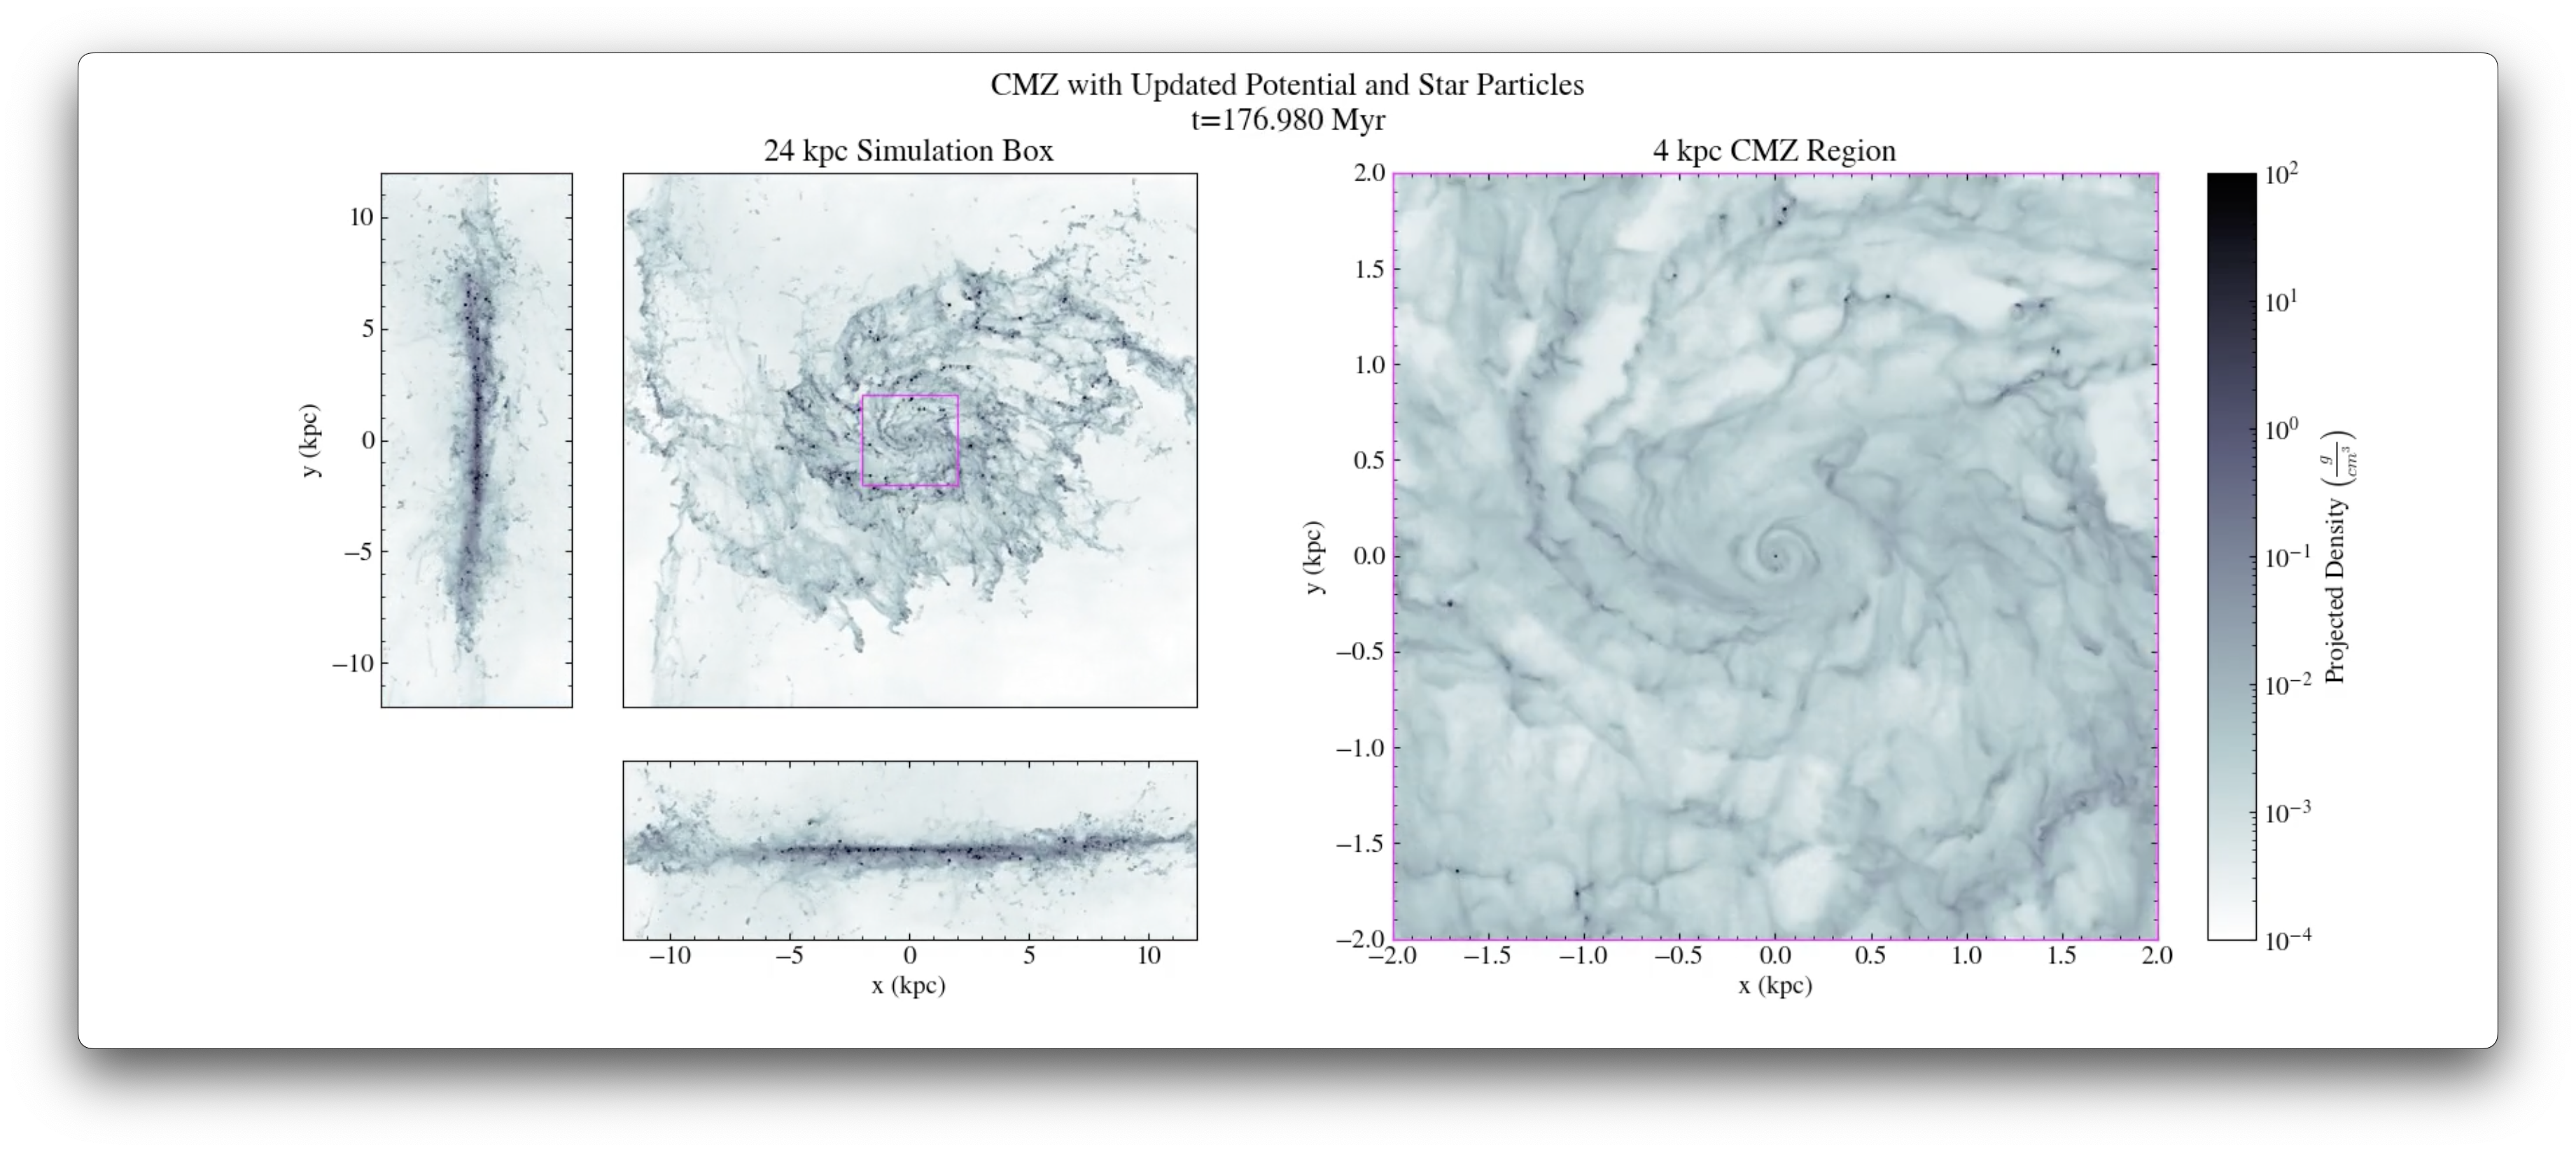
\includegraphics[width=0.9\linewidth]{cmz.png}
  \end{center}
  \end{columns}
\end{frame}
\placelogotrue
